
\section{Results}
The model with a 3-layers LSTM PyTorch cell has been trained on the 
Penn Tree-bank training set for 60 epochs, 
taking about 23 seconds per epoch and 23 minutes in total on a 
Nvidia Tesla T4.

Stochastic gradient descent (SGD) has been adopted as optimizer 
and the Cross-Entropy criterion as loss function.

The hyperparameters have been tuned on the validation set and 
the best hyperparameters found are shown in Table \ref{table:hyperparameters}.
A scheduler decays the learning rate of half every 20 epochs.

\begin{table}
\begin{center}
\begin{tabularx}{0.4\textwidth} { 
    | >{\centering\arraybackslash}X 
    | >{\centering\arraybackslash}X | }
   \hline
   \textbf{Hyperparameter} & \textbf{Value} \\
   \hline
   Batch size       & 128 \\
   Sequence length  & 40 \\
   Embedding size   & 200 \\
   Hidden size      & 250 \\
   Layers           & 3 \\
   Dropout cell     & 0.2 \\
   Dropout output   & 0.5 \\
   Clip value       & 0.2 \\
   Epochs           & 60 \\
   Learning rate    & 40 \\
  \hline
\end{tabularx}
\caption{Hyperparameters value.}
\label{table:hyperparameters}
\end{center}
\end{table}

\begin{figure}[ht]
\centerline{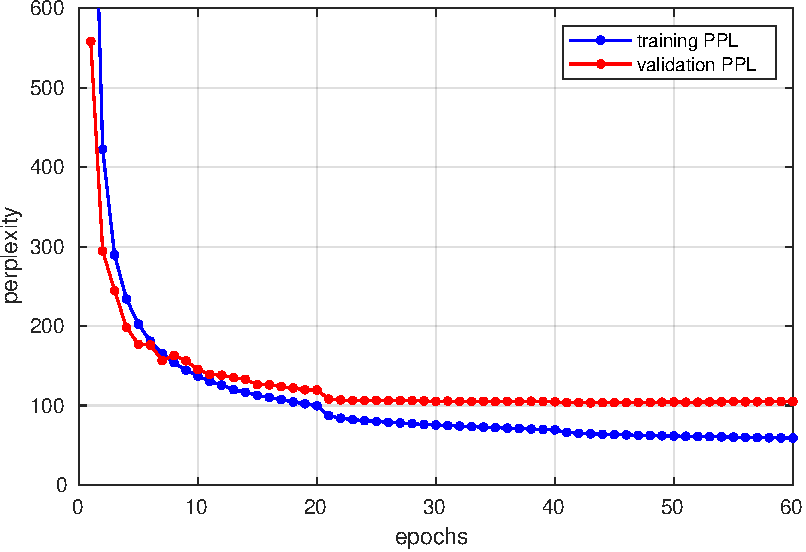
\includegraphics[scale=0.65]{ppl.pdf}}
\caption{Training and validation perplexity over the training process.}
\label{fig:PPL}
\end{figure}

\begin{figure}[ht]
\centerline{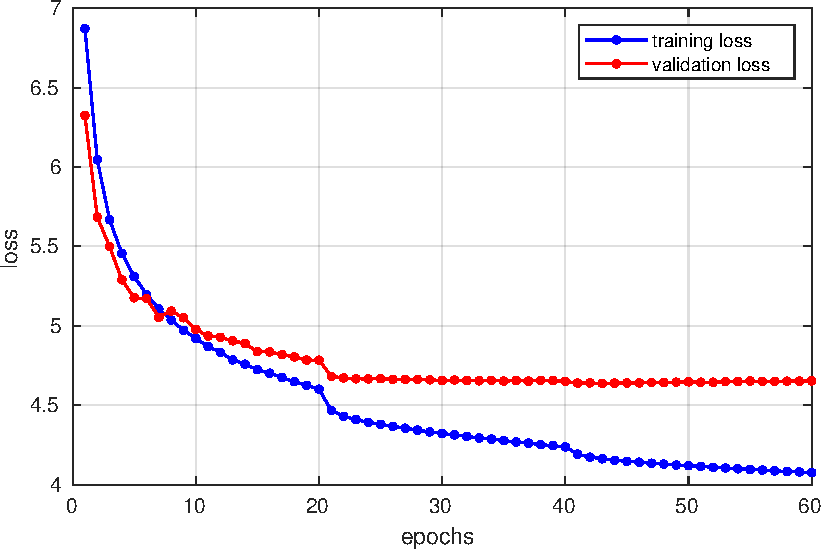
\includegraphics[scale=0.65]{loss.pdf}}
\caption{Training and validation loss over the training process.}
\label{fig:loss}
\end{figure}
    

Figure \ref{fig:PPL} shows the perplexity of training and validation and 
Figure \ref{fig:loss} shows the loss over the training process.
The best model, i.e. the one with the lowest validation perplexity during training, 
% has been evaluated on the test set obtaining a
obtains a perplexity equals to $98.8$ and $103.3$, respectively, on the 
test and validation set.
These results are not much higher than the performances reported by 
Zaremba et al. \cite{Zaremba}, i.e. a perplexity of $82.7$ and $86.2$, 
respectively, on the test and validation set.
